\documentclass[12pt, twoside]{article}
\usepackage[letterpaper, margin=1in, headsep=0.5in]{geometry}
\usepackage[english]{babel}
\usepackage[utf8]{inputenc}
\usepackage{amsmath}
\usepackage{amsfonts}
\usepackage{amssymb}
\usepackage{tikz}
%\usetikzlibrary{quotes, angles}

\usepackage{graphicx}
\usepackage{enumitem}
\usepackage{multicol}

\usepackage{fancyhdr}
\pagestyle{fancy}
\fancyhf{}
\renewcommand{\headrulewidth}{0pt} % disable the underline of the header

\fancyhead[RE]{\thepage}
\fancyhead[RO]{\thepage \\ Name: \hspace{3cm}}
\fancyhead[L]{BECA / Dr. Huson / 10th Grade Geometry\\* Unit 8 Transformations\\13 March 2019}

\begin{document}
\subsubsection*{8-6 Do Now: Transformation compositions}
  \begin{enumerate}
    \item Name the details required to completely specify each transformation.
    \begin{enumerate}
      \item Translation: Answer: the change in $x$ direction and in the $y$ direction
      \item Reflection: \vspace{0.8cm}
      \item Rotation: \vspace{0.8cm}
      \item Dilation:
    \end{enumerate} \vspace{0.5cm}

  \item Quadrilateral $ABCD$ undergoes two tranformations mapping it onto $A''B''C''D''$, as shown below. Specify the two tranformations in detail.
    \vspace{1.75cm}

      \begin{center} %4 quadrant regents grid w T-Chart
      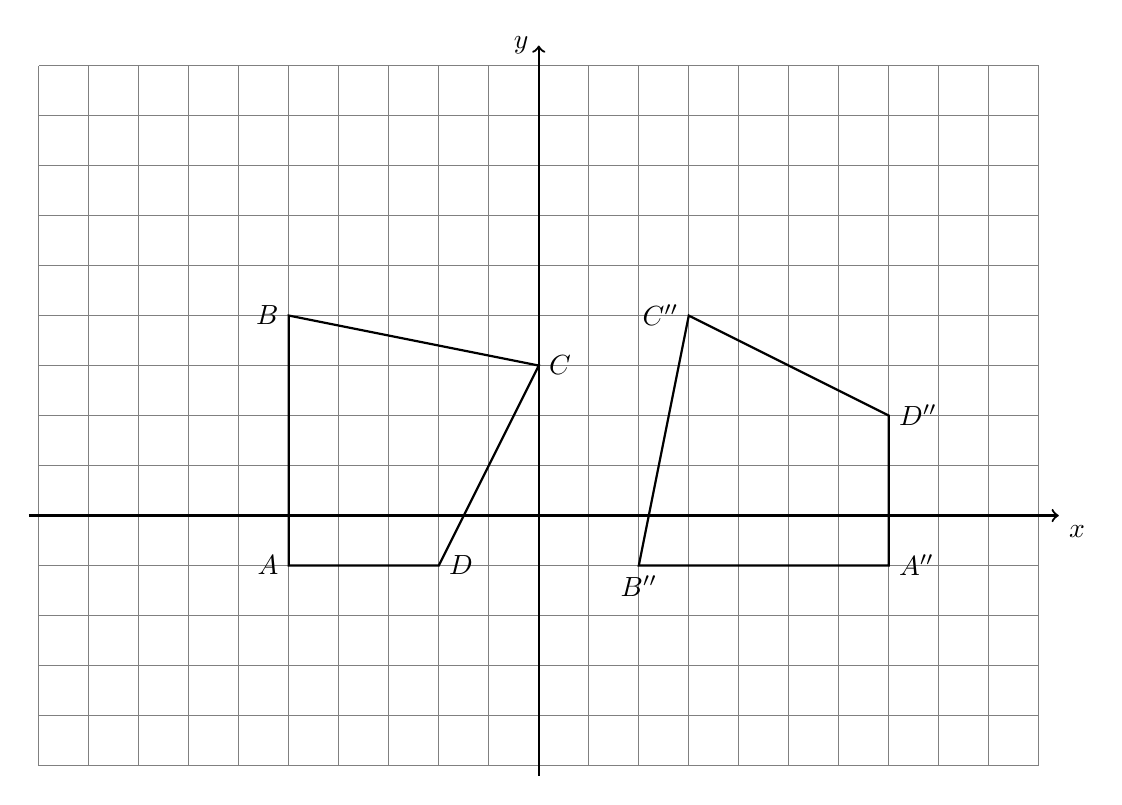
\begin{tikzpicture}[scale=.635]
        \draw [help lines] (-10,-5) grid (10,9);
        \draw [thick, ->] (-10.2,0) -- (10.4,0) node [below right] {$x$};
        \draw [thick, ->] (0,-5.2)--(0,9.4) node [left] {$y$};
        \draw [thick] (-5,-1)node[left]{$A$}--
          (-5,4)node[left]{$B$}--
          (0,3)node[right]{$C$}--
          (-2,-1)node[right]{$D$}--cycle;
        \draw [thick] (7,-1)node[right]{$A''$}--
          (2,-1)node[below]{$B''$}--
          (3,4)node[left]{$C''$}--
          (7,2)node[right]{$D''$}--cycle;
      \end{tikzpicture}
      \end{center}
    Rewrite each statement that is true and applies to this problem from the following list:
    \begin{itemize}
      \item Both transformations are rigid motions.
      \item The reflection preserves orientation.
      \item Lengths and angles are preserved so the quadrilaterals are congruent.
    \end{itemize}

  \end{enumerate}

  \end{document}
